\begin{figure*}[!h]
  \vspace{-0.7cm}
\center
\begin{tabular}{cccc}
% \hspace{-5.cm} \panel{A} & \hspace{-5.2cm}\panel{B}  \\[-0.2cm]
\raisebox{3.7cm}{\panel{A}} & 
\hspace{-0.5cm}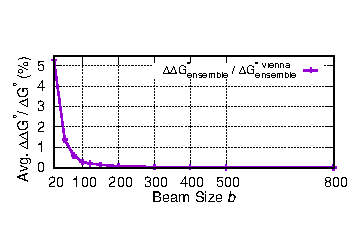
\includegraphics[width=0.4\textwidth]{figs/ensemble_beamsize_overall} &
\raisebox{3.7cm}{\panel{B}} &
\hspace{-0.5cm}{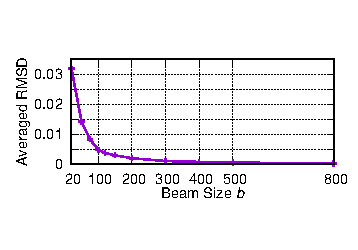
\includegraphics[width=0.4\textwidth]{figs/RMSD_beamsize_overall}}
\end{tabular}
\\[-1.2cm]
\begin{tabular}{c@{}c@{}c@{}c@{}c@{}c}
% \hspace{-5.cm}\panel{C} & \hspace{-5.2cm}\panel{D} & \hspace{-5.8cm}\panel{E} \\[-0.2cm]
\hspace{0.6cm}\raisebox{3.8cm}{\panel{C}} & 
\hspace{-1cm}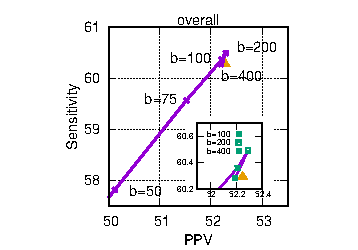
\includegraphics[width=.35\textwidth]{figs/precision-recall-overall-lpv} 
&
\hspace{-.5cm}\raisebox{3.8cm}{\panel{D}} & 
\hspace{-1.2cm}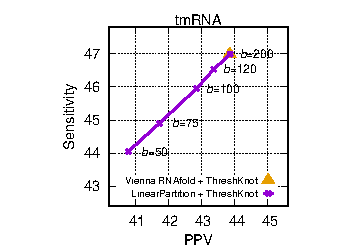
\includegraphics[width=0.35\textwidth]{figs/precision-recall-tmRNA-lpv-hzhang}
&
\hspace{-0cm}\raisebox{3.8cm}{\panel{E}} & 
\hspace{-1.5cm}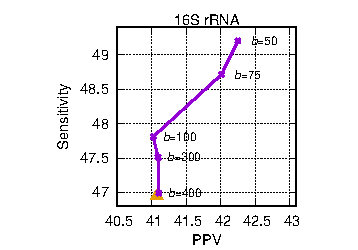
\includegraphics[width=0.35\textwidth]{figs/precision-recall-16s-lpv-hzhang}
\vspace{-0.4cm}
\end{tabular}
\caption{
Impact of beam size. 
{\bf A}: Relative difference of 
  ensemble folding free energy change, $\ddg/\Delta G^\circ_\text{ensemble}$, against  beam size. %, averaged over all families.
{\bf B}: RMSD against beam size. %, averaged over all families.
{\bf C}: Overall PPV and Sensitivity with beam size.
{\bf D--E}: tmRNA and 16S rRNA PPV and Sensitivity against beam size, respectively. 
%{\bf E}: 16S rRNA PPV and Sensitivity change with beam size. 
Note that the  results of \threshknot using \rnafold (yellow triangles in {\bf C--E}) are identical to \threshknot using
the {\em exact} version of \linearpartition ($b\!=\!\infty$).
%since \linearpartition with infinite beam size (i.e., no beam pruning) does $O(n^3)$ exact partition function calculation as \viennarnafold.
\label{fig:beamsize}
\vspace{-0.7cm}
}
\end{figure*}
